% ============================================================
%  Chapter 3 — Proposed System Architecture & Design
% ============================================================

\section{System Architecture}

The SmartGrid AI Audit Framework is a modular cyber-physical monitoring and audit platform that puts anomaly detection, audit decision support, explainability, and operator-facing visualisation into one system. The design builds on the conceptual foundation laid by Priyadarsini~\cite{priyadarsini2025}, who proposed coupling anomaly detection with audit scheduling in multi-agent smart grids, and extends it into a fully operational implementation. The architecture is organised around two distinct operational workspaces: \textit{Experiment Running}, which serves as the simulation and benchmarking environment; and \textit{Rapid SCADA Live}, which provides real-time monitoring over a live supervisory control and data acquisition (SCADA) infrastructure~\cite{martinelli2022method}. This split keeps experimental validation independent of the production monitoring pipeline, while both workspaces share the same detection, scoring, and audit logic.

\par \vspace{0.35cm}
The system is structured into four functional tiers. Tier~1 handles data ingestion and integration, bringing heterogeneous telemetry streams into a common format. Tier~2 performs feature processing and baseline mapping, converting raw observations into normalised cyber-physical feature vectors. Tier~3 runs the multi-layer anomaly detection engine and audit intelligence module, combining statistical, temporal, and attack-specific detectors with a hybrid scheduling mechanism. Tier~4 provides the visualisation and operator interface through a web-based dashboard. Figure~\ref{fig:flow_architecture} shows the end-to-end architecture, and Figure~\ref{fig:tier_architecture} illustrates the four-tier layout.

\begin{figure}[H]
\centering
\fbox{\includegraphics[width=0.95\textwidth]{Flow.png}}
\caption{End-to-end architecture of the SmartGrid AI Audit Framework.}
\label{fig:flow_architecture}
\end{figure}

\begin{figure}[H]
\centering
\fbox{\includegraphics[width=0.95\textwidth]{TierArchitecture.png}}
\caption{Four-tier scientific architecture of the proposed system.}
\label{fig:tier_architecture}
\end{figure}

\begin{figure}[H]
\centering
\fbox{\includegraphics[width=0.95\textwidth]{dettailed_architecture.png}}
\caption{Detailed component-level architecture showing the internal modules and data flow between subsystems.}
\label{fig:detailed_architecture}
\end{figure}

% ------------------------------------------------------------
\subsection{Tier 1: Data Ingestion and Integration Layer}
% ------------------------------------------------------------

The data ingestion layer is responsible for acquiring telemetry from two independent sources and unifying them into a common representation suitable for downstream processing.

\par \vspace{0.35cm}
\textbf{Experiment Data Stream.} The experiment workspace operates on pre-configured simulation scenarios that generate cyber-physical observations for a parameterised number of agents over a defined number of timesteps. This stream is used exclusively for benchmarking, method comparison, and controlled evaluation of detection and audit algorithms. The experiment data is produced by the backend simulation engine, which models both normal operating conditions and injected attack scenarios.

\par \vspace{0.35cm}
\textbf{Rapid SCADA Live Stream.} The live workspace interfaces with a Rapid SCADA deployment that manages a fixed grid of 100 agents distributed across four asset classes~\cite{farid2014multi}:

\begin{itemize}
    \item \textbf{Generators (GEN-01 to GEN-20):} Each generator agent reports five physical measurements (voltage, frequency, current, power, and response time) and four cyber indicators (latency, packet loss, integrity, and communication frequency). These 20 agents represent the primary power generation units of the simulated grid and carry 7 SCADA channels each (3 physical + 4 cyber).
    \item \textbf{Substations (SUB-21 to SUB-50):} Each substation agent reports five physical measurements (voltage as substation load, frequency, current as physical latency, power, and response time) and three cyber indicators (packet loss, integrity, and communication frequency). SUB agents have no dedicated SCADA latency channel; the bridge fills a nominal latency value ($\approx 0.15$) with jitter. These 30 agents carry 6 SCADA channels each (3 physical + 3 cyber).
    \item \textbf{Phasor Measurement Units (PMU-51 to PMU-75):} Each PMU agent reports five physical measurements (voltage, frequency, current, power, and response time) and four cyber indicators (latency, packet loss, integrity, and communication frequency). These 25 agents provide high-resolution synchronised measurements of grid state and carry 7 SCADA channels each.
    \item \textbf{Breakers (BRK-76 to BRK-100):} Each breaker agent reports five physical measurements, status (mapped to voltage: 1.0 = closed), fault count (mapped to current), frequency, power, and response time, and four cyber indicators (latency, packet loss, integrity, and communication frequency). These 25 agents represent the protective switching devices of the grid and carry 7 SCADA channels each.
\end{itemize}

A PowerShell-based bridge script retrieves SCADA telemetry through the Rapid SCADA Web API using authenticated HTTP requests. The bridge polls the SCADA server at configurable intervals, collects the current channel values for all 100 agents, and forwards the data to the FastAPI backend in batch form. The SCADA values in the current deployment are produced by calculated channels configured within Rapid SCADA rather than by physical field instrumentation. This design choice allows full end-to-end system integration and validation while keeping the data provenance transparent.

\par \vspace{0.35cm}
\textbf{Data Unification.} Regardless of origin, both data streams are transformed into standardised cyber-physical feature vectors before entering the processing pipeline. Each agent observation at each timestep is represented as a fixed-length vector comprising physical measurements and cyber-network indicators. This way, all downstream detection, scoring, and audit modules work on the same data format.

\begin{figure}[H]
\centering
\fbox{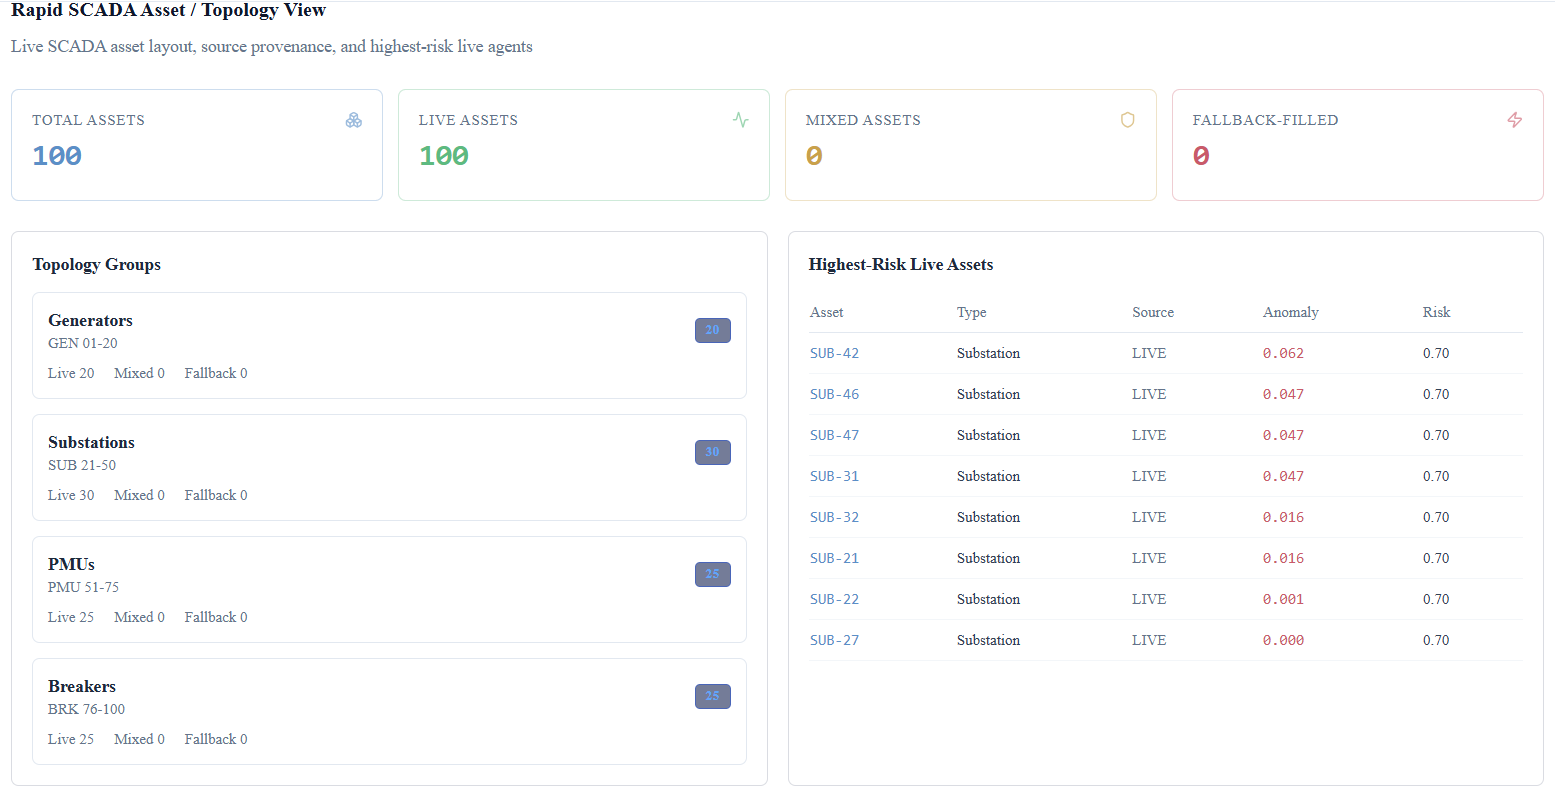
\includegraphics[width=0.95\textwidth]{FigRapid_SCADA_Asset_Topology_View.png}}
\caption{Rapid SCADA asset topology view showing the 100-agent grid layout across four asset classes.}
\label{fig:scada_topology}
\end{figure}

% ------------------------------------------------------------
\subsection{Tier 2: Feature Processing and Baseline Mapping}
% ------------------------------------------------------------

The feature processing tier transforms raw telemetry into normalised deviation vectors that quantify how far each observation departs from its expected baseline. The feature space is divided into two complementary domains.

\par \vspace{0.35cm}
\textbf{Physical Features.} Physical features capture the electrical and operational state of each agent and include measurements such as voltage, current, frequency, power, and response time. These features reflect the behaviour of the underlying physical infrastructure and are the primary indicators of grid health.

\par \vspace{0.35cm}
\textbf{Cyber Features.} Cyber features capture the communication and network state of each agent and include measurements such as latency, packet loss, communication frequency, and data integrity. These features reflect the health of the supervisory communication network and serve as indicators of potential cyber intrusions or network degradation.

\par \vspace{0.35cm}
\textbf{Baseline Specification.} Baselines are type-specific and hand-engineered for each asset class. Each feature within each asset type has a defined nominal baseline value and an associated threshold that represents the acceptable range of deviation. The baselines encode domain knowledge about normal operating conditions for generators, substations, PMUs, and breakers respectively. Table~\ref{tab:gen_baseline} illustrates the baseline profile for the generator (GEN) asset class as a representative example.

\begin{table}[H]
\centering
\caption{Generator (GEN) baseline profile: nominal values and thresholds.}
\label{tab:gen_baseline}
\begin{tabular}{llcc}
\hline
\textbf{Domain} & \textbf{Feature} & \textbf{Baseline ($b$)} & \textbf{Threshold ($\tau$)} \\
\hline
Physical & Voltage     & 230.0 V   & 10.0 V  \\
Physical & Frequency   & 50.0 Hz   & 1.0 Hz  \\
Physical & Current     & 100.0 A   & 20.0 A  \\
Physical & Power       & 23.0 kW   & 5.0 kW  \\
Physical & Response Time & 3.3 ms  & 5.0 ms  \\
\hline
Cyber    & Latency       & 0.17 (ratio) & 0.5  \\
Cyber    & Packet Loss   & 0.004       & 0.05 \\
Cyber    & Integrity     & 0.99        & 0.2  \\
Cyber    & Comm Frequency & 0.79       & 0.5  \\
\hline
\end{tabular}
\end{table}

\par \vspace{0.35cm}
\textbf{All Asset-Class Baseline Profiles.} Table~\ref{tab:gen_baseline} showed the GEN profile. The remaining three asset classes each carry distinct calibrated baselines that reflect their different operational roles within the grid. Table~\ref{tab:all_baselines} presents the complete per-type nominal baseline values for the key physical and cyber features across all four classes.

\begin{table}[H]
\centering
\caption{Per-type baseline profiles for all four agent classes: nominal values for primary features.}
\label{tab:all_baselines}
\renewcommand{\arraystretch}{1.25}
\begin{tabular}{|l|c|c|c|c|c|c|}
\hline
\textbf{Agent Class} & \textbf{Voltage (V)} & \textbf{Current (A)} & \textbf{Latency} & \textbf{Pkt Loss} & \textbf{Integrity} & \textbf{Comm Freq} \\
\hline
GEN & 231.0 & 13.0 & 0.17 & 0.003 & 0.99 & 0.80 \\
\hline
SUB & 189.0 (load) & 4.0 & 0.15 & 0.003 & 0.98 & 0.78 \\
\hline
PMU & 231.0 & 100.0 & 0.12 & 0.003 & 0.99 & 0.81 \\
\hline
BRK & 1.0 (status) & 0.0 & 0.17 & 0.004 & 0.99 & 0.80 \\
\hline
\end{tabular}
\end{table}

\par \vspace{0.25cm}
\noindent
The profiles encode the different physical roles of each class. Substations report a lower voltage (189~V as load-side) and a much lower current (4~A) compared with generators. PMUs report very high current (100~A) because they measure line current at the transmission level, and they have a lower latency baseline (0.12) reflecting their high-frequency synchronised measurement rate. Breakers report a voltage of 1.0 mapped to status (1 = closed, 0 = open) and zero current because they are switching devices rather than energy carriers. Using separate per-type baselines rather than a single fleet-wide average prevents the deviation scorer from systematically flagging breakers for having near-zero current, or PMUs for having high current, which is the normal condition for each class.

\par \vspace{0.35cm}
\textbf{Normalisation.} Each observed feature value is normalised against its baseline using the following transformation:
\begin{equation}
z_{j} = \frac{x_{j} - b_{j}}{\tau_{j}}
\label{eq:normalisation}
\end{equation}
where $x_{j}$ is the observed value of feature $j$, $b_{j}$ is the baseline value, and $\tau_{j}$ is the threshold. The resulting normalised value $z_{j}$ expresses the observation as a multiple of its acceptable deviation, which allows direct comparison across different feature types and asset classes.

% ------------------------------------------------------------
\subsection{Tier 3: Multi-Layer Anomaly Detection and Audit Intelligence}
% ------------------------------------------------------------

Tier~3 is the core analytical engine of the framework. It comprises multiple detection layers that operate in concert to identify anomalies, classify attack types, produce risk scores, determine audit actions, and generate human-readable explanations. The following subsections describe each component in detail.

\par \vspace{0.35cm}
\textbf{Statistical Deviation Scoring.}

\par \vspace{0.2cm}
The statistical deviation scorer computes a weighted composite score for each agent at each timestep by measuring the root-mean-square deviation of physical and cyber features from their respective baselines~\cite{priyadarsini2025}. For agent $i$ at time $t$, the deviation score is computed as:
\begin{equation}
S_{i}(t) = w_{i} \left( d_{x} + d_{y} \right)
\label{eq:deviation_score}
\end{equation}
where $d_{x}$ and $d_{y}$ denote the physical and cyber deviation components respectively. The physical deviation is defined as:
\begin{equation}
d_{x} = \sqrt{ \frac{1}{n_{x}} \sum_{j=1}^{n_{x}} \left( \frac{x_{j} - b_{x,j}}{\tau_{x,j}} \right)^{2} }
\label{eq:physical_deviation}
\end{equation}
where $n_{x}$ is the number of physical features, $x_{j}$ is the observed value, $b_{x,j}$ is the physical baseline, and $\tau_{x,j}$ is the physical threshold. The cyber deviation $d_{y}$ is computed analogously over the cyber feature set. The weight $w_{i}$ captures the relative importance of agent $i$ in the grid topology and can be adjusted to reflect criticality.

\par \vspace{0.35cm}
\textbf{LSTM Temporal Detector.}

\par \vspace{0.2cm}
The LSTM-based temporal detector is designed to capture sequential dependencies in agent behaviour that may not be apparent from instantaneous deviation scores alone. The detector employs a dual-branch architecture comprising a physical grid branch and a network/cyber branch. Each branch processes a sliding window of the most recent timesteps, producing a representation of the agent's recent temporal trajectory. In the experiment workspace, each branch receives 3 physical and 4 cyber features (7 total) as defined by the simulation environment; in the SCADA live workspace, each branch receives 5 physical and 4 cyber features (9 total) as provided by the SCADA adapter's type-specific feature mapping.

\par \vspace{0.2cm}
The two branch outputs are fused in a first-stage operation using fixed weights ($w_{\text{grid}} = 0.58$, $w_{\text{network}} = 0.42$) to produce a single calibrated anomaly probability $p_{\text{fused}}$. The grid branch carries the higher weight because physical instability is the primary threat surface in the power grid context. Temperature scaling is applied to the raw output logits before the sigmoid activation to ensure that the resulting probability is well-calibrated. This Stage~1 fusion happens entirely within the LSTM module, before the output is passed on to the ensemble layer.

\par \vspace{0.35cm}
\textbf{Stage~2 Weighted Ensemble Fusion.}

\par \vspace{0.2cm}
It is important to distinguish this second-stage fusion from the Stage~1 dual-branch fusion described above. Stage~1 fuses the two LSTM branches (physical vs.\ cyber) to produce a single probability. Stage~2 fuses two entirely different evidence sources, the statistical deviation scorer and the LSTM-based temporal detector, to produce a hybrid confidence estimate. The Stage~2 ensemble combines $p_{\text{fused}}$ from Stage~1 with the deviation-derived confidence to form the final decision signal. The deviation score and the fused LSTM probability are combined through a weighted ensemble to produce a hybrid confidence value for each agent at each timestep:
\begin{equation}
\text{hybrid\_conf}_{i}(t) = w_{\text{dev}} \cdot \text{dev\_conf}_{i}(t) + w_{\text{prob}} \cdot \text{prob\_support}_{i}(t) + \text{suspicion\_credit}_{i}(t)
\label{eq:hybrid_conf}
\end{equation}
where $w_{\text{dev}} = 0.48$ and $w_{\text{prob}} = 0.52$ are the ensemble weights for the deviation-based confidence and the LSTM probability support respectively. The suspicion credit term accumulates evidence over time for agents that exhibit borderline behaviour: each timestep in which an agent's LSTM probability exceeds a soft threshold adds a small increment to the credit, while consecutive normal readings decay the credit back toward zero. This way, agents with repeated borderline readings get escalated over time, even when no single observation on its own is decisive. The binary anomaly flag is triggered only when multiple conditions from both the deviation and probability branches agree:
\begin{equation}
a_{i}(t) =
\begin{cases}
1 & \text{if deviation AND probability conditions are satisfied} \\
0 & \text{otherwise}
\end{cases}
\label{eq:anomaly_flag}
\end{equation}

Requiring both detectors to agree prevents isolated spikes in either the statistical or temporal detector from triggering false positives.

\par \vspace{0.35cm}
\textbf{Multi-Layer Multi-Detector Architecture.}

\par \vspace{0.2cm}
Beyond the ensemble fusion, the system implements a multi-layer detection architecture that provides specialised detection capabilities for different attack and fault types. Each layer operates independently and contributes to the final anomaly determination through an OR-with-precedence combiner. Figure~\ref{fig:layerc_arch_ch3} shows the full layout including the four Layer C sub-detectors.

\begin{figure}[H]
\centering
\fbox{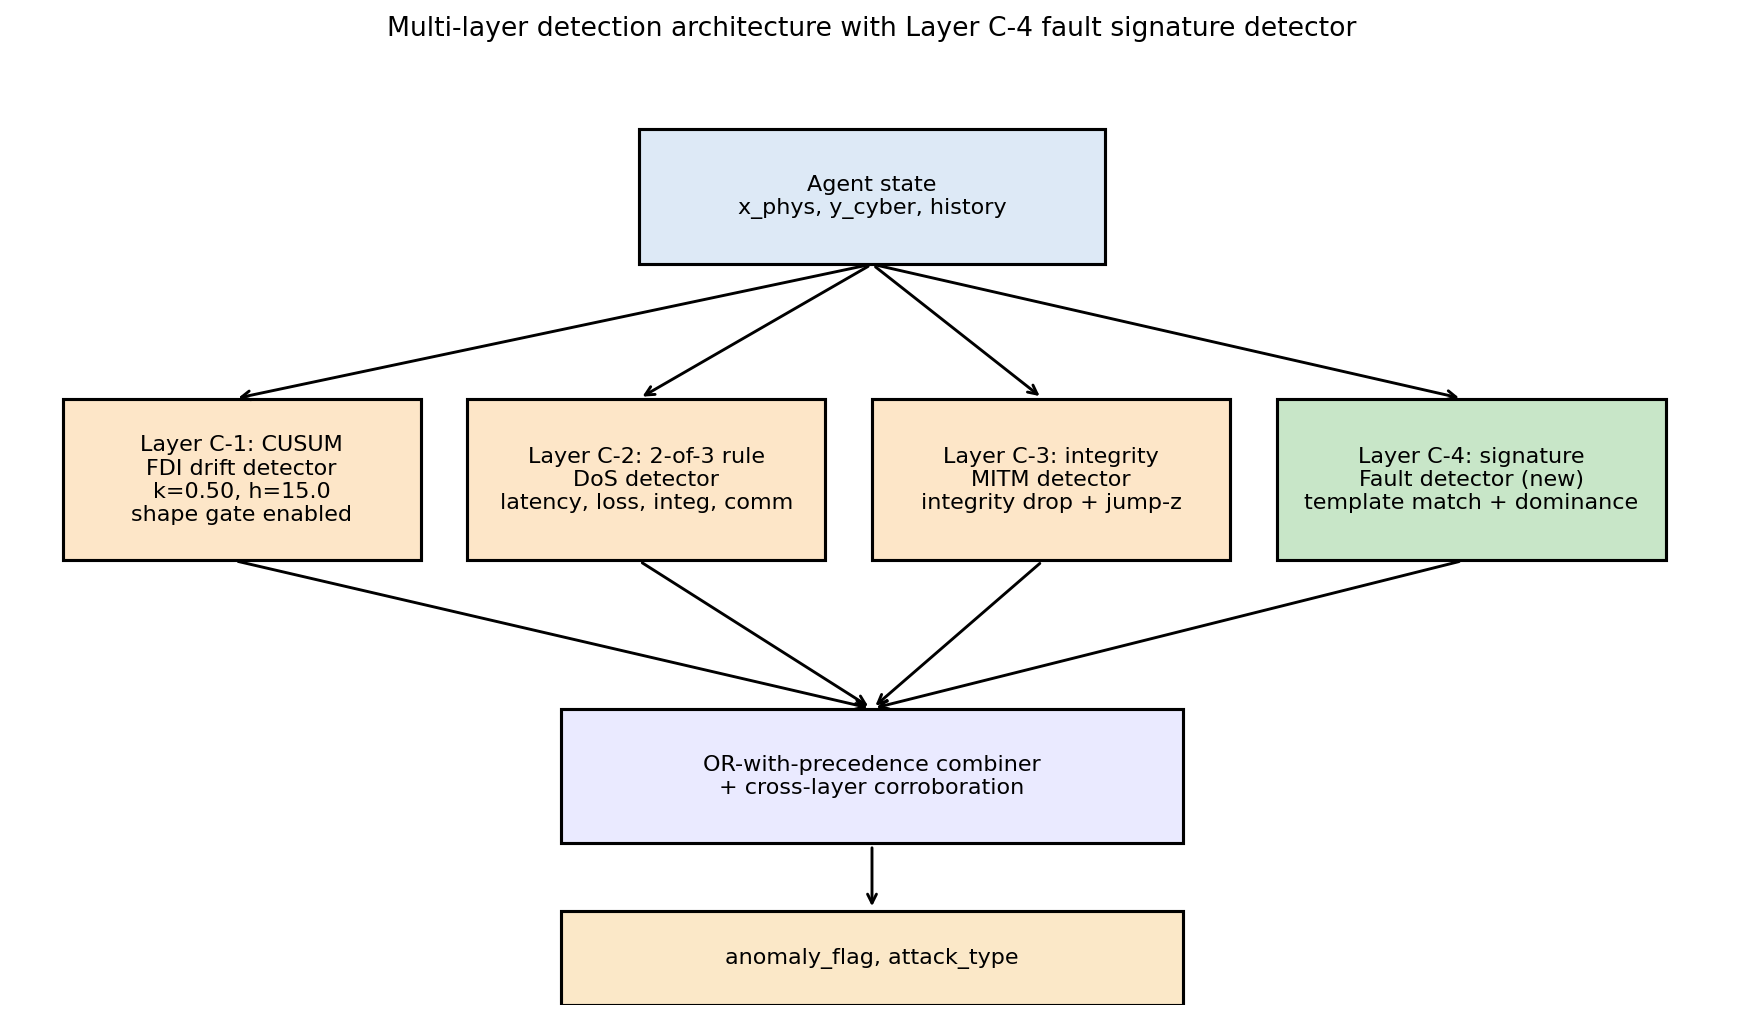
\includegraphics[width=0.95\textwidth]{Fig_LayerC_Architecture.png}}
\caption{Multi-layer detection architecture. The agent state feeds the four Layer C sub-detectors (CUSUM for FDI, 2-of-3 for DoS, integrity jump for MITM, and signature template for faults). Their outputs are merged by an OR-with-precedence combiner with cross-layer corroboration.}
\label{fig:layerc_arch_ch3}
\end{figure}

\par \vspace{0.2cm}
\textit{Layer A, Calibrated LSTM Threshold.} Layer~A applies a strict threshold on the calibrated LSTM output. An agent is flagged by this layer when its predicted anomaly probability satisfies $p \geq 0.80$ and its deviation score satisfies $S \geq 3.60$. This layer captures high-confidence anomalies where both the temporal model and the statistical scorer independently indicate strong evidence of deviation.

\par \vspace{0.2cm}
\textit{Layer B, Temporal Accumulator.} Layer~B implements a sustained suspicion detector that flags agents exhibiting moderate but persistent anomalous behaviour. An agent is flagged by this layer when its LSTM anomaly probability exceeds $p \geq 0.55$ for at least 5 consecutive timesteps within a rolling window of 6 timesteps. This layer is designed to detect slow-onset or gradually escalating anomalies that may not trigger the high-confidence threshold of Layer~A at any individual timestep but collectively represent a sustained departure from normal behaviour. Layer~B is operational in the current implementation, but an earlier design explored a second suppression tier (Tier-B) sitting between Layer~A and Layer~C to apply additional corroboration filtering. Multiple variants of Tier-B were evaluated, criticality-weighted gating, anomaly-spike-based gating, and percentile-based filtering, and all variants were found to reduce the false positive rate only marginally while producing a measurable drop in recall. The operating point of 94.23\% per-step accuracy with 100\% aggregate recall was judged to be more defensible than any Tier-B configuration tested, so Tier-B was removed and the architecture settled on the current three-layer layout (Layer~A, Layer~B, Layer~C).

\par \vspace{0.2cm}
\textit{Layer C: Attack and Fault Specific Detectors.} Layer~C comprises four specialised sub-detectors, each targeting a specific class of cyber-physical attack or physical fault:

\begin{itemize}
    \item \textbf{Layer C-1: CUSUM Drift Detector with Shape Gate (FDI).} This detector implements a two-sided cumulative sum on the physical residuals. The algorithm uses sensitivity $k = 0.50$ and alarm threshold $h = 15.0$ over a sliding window of 8 consecutive timesteps. Beyond the cumulative test, a shape gate is applied at the most recent step: at least two of the three FDI signature directions ($z[0] > 0.5$, $z[1] > 0.5$, $z[2] < -0.5$) must agree before the layer fires. This filter removes cumulative drifts that come from random noise rather than a coherent FDI signature, while keeping the layer responsive to real injections whose residual already matches the multi feature pattern~\cite{liu2009false}\cite{yan2020false}.

    \item \textbf{Layer C-2: Network Rule Detector for Denial of Service (DoS).} A weighted score is computed across all four cyber features (latency ratio, packet loss, integrity drop, and communication drop), with weights $0.20, 0.30, 0.30, 0.20$ respectively. The layer fires when the weighted score exceeds $0.45$, with a guard that suppresses the fire when integrity dominates and latency or packet loss are both weak (in that case the event is left to Layer C-3). This rule based formulation reduces false positives arising from transient network congestion.

    \item \textbf{Layer C-3: Integrity and Temporal Jump Detector for MITM.} The layer combines two signals~\cite{sadeghi2015security}: an integrity drop of at least $35\%$ from baseline, and a baseline aware jump z score of at least $2.5\sigma$. A guard vetoes the fire when latency and packet loss are both elevated (a DoS pattern). Both signals are required, which keeps precision high against legitimate operational transients.

    \item \textbf{Layer C-4: Signature Template Detector for Physical Faults (new contribution).} The layer template matches the physical residual against the three documented fault signatures (voltage sag, overcurrent, frequency deviation). It uses a primary z floor of $2.2$, a dominance ratio of $2.0$ between the primary feature and the strongest other feature, and a cyber guard of $2.5$ that vetoes the fire whenever any cyber channel deviates strongly (which would indicate a cyber attack rather than a physical fault). The detector fills a gap in the earlier architecture, where physical faults relied on fallback signature matching from the deviation pipeline and were frequently mistyped as FDI; with C-4 in place, the FAULT class is now identified with the same per type confidence as the cyber attack classes.
\end{itemize}

\par \vspace{0.2cm}
\textit{Combiner: OR-with-Precedence and Cross-Layer Corroboration.} The outputs of all layers are combined using an OR-with-precedence rule: if any layer fires, the agent is flagged as anomalous. When multiple layers fire simultaneously, the layer with the highest specificity (Layer~C, then Layer~A, then Layer~B) takes precedence for attack classification, and within Layer~C the new fault detector (C-4) takes precedence over CUSUM (C-1) when both fire on the same step, because the C-4 fire requires single feature dominance and quiet cyber channels, which is direct evidence against the FDI shape. A cross-layer corroboration gate is also applied after the per layer decisions: a flag raised purely by the deviation magnitude path (the severe deviation trigger) with low LSTM confidence ($p < 0.45$) and no Layer~C agreement is demoted to a clean prediction. This single rule removes the dominant noise driven false positive pattern without affecting any case where at least one detector signature is present.

\par \vspace{0.2cm}
\textit{Temporal Signature Classification.} Alongside the three-layer detectors, a lightweight temporal pattern classifier analyses the shape of the deviation trajectory over the most recent five timesteps to identify the physical signature of the anomaly. Four signature types are recognised:
\begin{itemize}
    \item \textbf{STEP}, an abrupt, sustained shift in one or more features (characteristic of FDI with a constant bias).
    \item \textbf{RAMP}, a linearly increasing deviation over time (characteristic of FDI with a drift component, or gradual load faults).
    \item \textbf{OSCILLATORY}, alternating positive and negative deviations with no persistent direction (characteristic of MITM measurement noise or sensor interference).
    \item \textbf{STABLE}, no significant change pattern detected (consistent with normal operation or a very slow developing fault).
\end{itemize}
The classified signature feeds into the five-class attack typing module described below, providing an additional discriminative signal beyond the instantaneous feature values.

\par \vspace{0.2cm}
\textit{Five-Class Attack Typing.} The system assigns each flagged agent one of five attack class labels using a weighted combination of the Layer~C detector outputs, the temporal signature, and the deviation magnitudes across physical and cyber domains:
\begin{itemize}
    \item \textbf{FDI (False Data Injection):} Physical features show a STEP or RAMP signature; CUSUM detector fires; cyber features are within normal range.
    \item \textbf{DOS (Denial of Service):} Network rule detector fires; latency, packet loss, and communication frequency conditions are triggered; physical features are largely unaffected.
    \item \textbf{MITM (Man-in-the-Middle):} Integrity-jump detector fires; OSCILLATORY signature present; both physical and cyber features show simultaneous noise.
    \item \textbf{FAULT (Physical Equipment Fault):} Physical features show large deviations consistent with hardware failure (voltage collapse, current spike); cyber features remain healthy; no network rule or MITM indicator present.
    \item \textbf{CHAIN (Coordinated Cross-Layer Attack):} Multiple Layer~C detectors fire simultaneously; both physical and cyber deviations are elevated; indicates a coordinated attack targeting multiple system layers at once.
\end{itemize}
The attack type label is reported alongside the anomaly flag in both the audit trail and the explainability output, so operators know not only that an anomaly was detected but also what class of event the system believes it is dealing with.

\par \vspace{0.2cm}
\textit{Tier-A False Positive Suppression.} To reduce spurious alerts, a suppression mechanism is applied at the output stage. An alert is suppressed only when all five of the following conditions are simultaneously satisfied: the score ratio falls below 3.50, the LSTM anomaly probability is below 0.60, the network intrusion probability is below 0.55, the hybrid confidence is below 1.05, and no behavioural signature from the Layer~C detectors is present. Requiring all five conditions to hold together ensures that only genuine low-evidence detections are suppressed. If any single condition is not met, for instance, the LSTM probability is elevated even when the score ratio is low, the alert is retained and passed through to the operator.

\begin{figure}[H]
\centering
\fbox{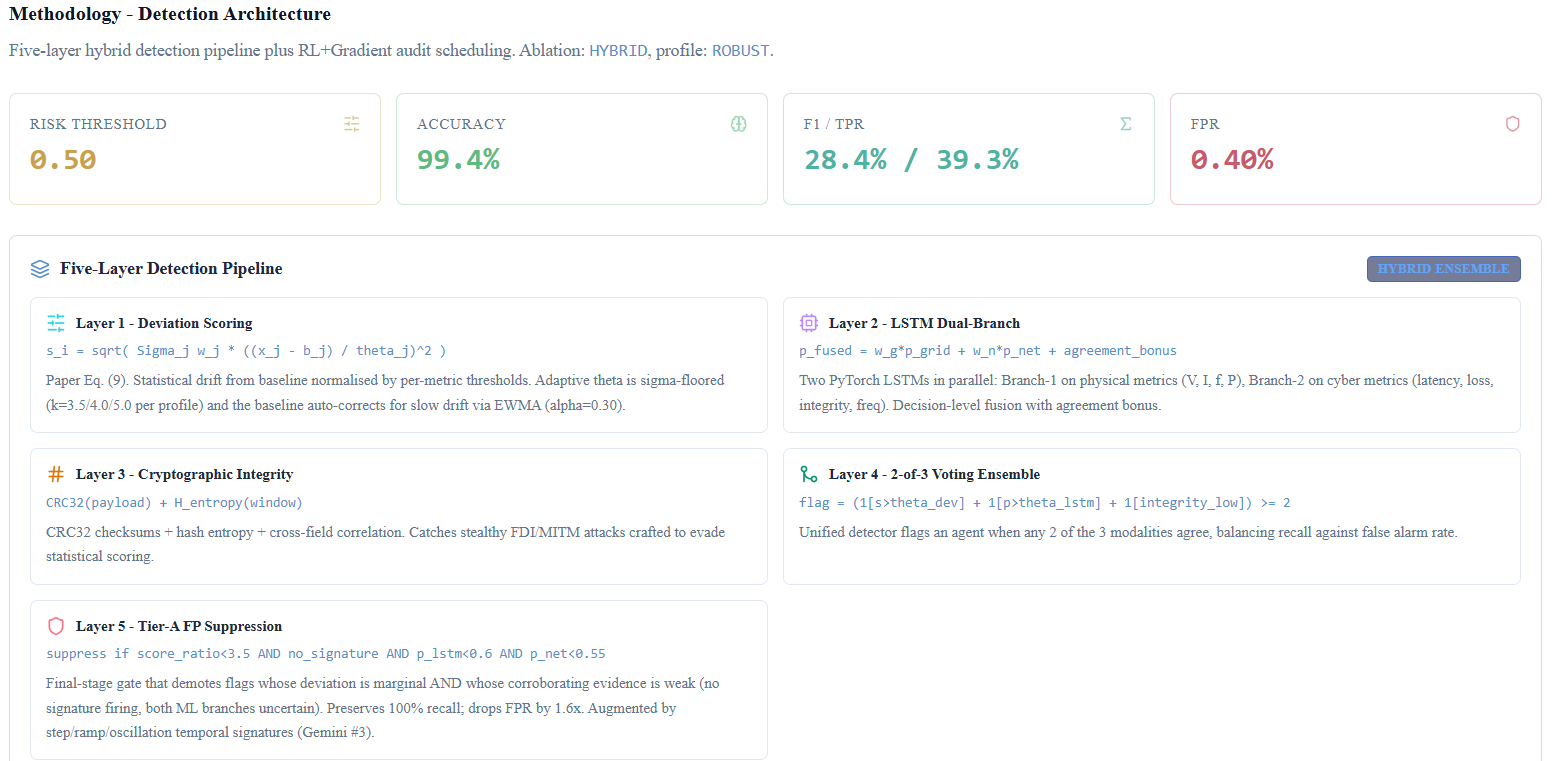
\includegraphics[width=0.95\textwidth]{FigMethodology_-_Detection_Architecture.png}}
\caption{Multi-layer detection architecture showing the three detection layers and the OR-with-precedence combiner.}
\label{fig:detection_architecture}
\end{figure}

\par \vspace{0.35cm}
\textbf{Audit Decision Logic.}

\par \vspace{0.2cm}
The audit decision module determines the appropriate audit frequency and escalation action for each agent based on the detection outputs and a hybrid optimisation strategy. The module combines reinforcement learning with gradient-based cost optimisation to balance detection effectiveness against audit cost.

\par \vspace{0.2cm}
\textit{Hybrid Scheduler.} The scheduler employs Q-learning~\cite{priyadarsini2025,ibrahim2023security} to adjust audit frequencies in response to observed anomaly patterns. The Q-learning agent maintains a state representation that encodes the current risk level and audit history of each grid agent, and selects actions that maximise a reward function balancing detection coverage and resource efficiency.

\par \vspace{0.2cm}
\textit{Cost Function.} The audit cost for agent $i$ operating at audit frequency $f_{i}$ is defined as:
\begin{equation}
C_{i} = C_{a} \cdot f_{i} + C_{f} \cdot \frac{R_{i}}{f_{i}}
\label{eq:cost_function}
\end{equation}
where $C_{a}$ is the per-audit cost, $C_{f}$ is the cost associated with undetected failures, and $R_{i}$ is the risk score of agent $i$. The first term penalises excessive auditing, while the second term penalises insufficient auditing of high-risk agents. The optimal audit frequency is obtained by differentiating the cost function with respect to $f_{i}$:
\begin{equation}
\frac{\partial C_{i}}{\partial f_{i}} = C_{a} - C_{f} \cdot \frac{R_{i}}{f_{i}^{2}}
\label{eq:cost_gradient}
\end{equation}

Setting this gradient to zero yields the analytically optimal frequency, which the gradient-based component uses to guide the Q-learning policy toward cost-efficient solutions.

\par \vspace{0.2cm}
\textit{Action Escalation.} Based on the combined risk assessment from the detection layers and the audit scheduler, the system assigns one of five escalation actions to each agent:

\begin{itemize}
    \item \textbf{NO\_ANOMALY:} The agent is operating within normal parameters. Standard monitoring continues at the baseline audit frequency.
    \item \textbf{LOG\_MONITOR:} A marginal deviation has been observed. The event is logged and the agent is placed under enhanced passive monitoring without changing the audit frequency.
    \item \textbf{INCREASE\_AUDIT:} Elevated risk has been detected. The audit frequency for the agent is increased to improve monitoring granularity.
    \item \textbf{ISOLATE\_NOTIFY:} A confirmed anomaly has been detected with high confidence. The agent is flagged for isolation and the operator is notified for manual review.
    \item \textbf{EMERGENCY\_SHUTDOWN:} A critical threat has been identified with sustained high-confidence evidence. The system recommends immediate shutdown of the affected agent and alerts the operator through the highest-priority notification channel.
\end{itemize}

Budget constraints are enforced throughout the scheduling process to ensure that the total audit cost across all agents does not exceed the allocated operational budget.

\par \vspace{0.35cm}
\textbf{Explainability.}

\par \vspace{0.2cm}
The explainability module generates per-agent, per-timestep explanations that identify the specific features contributing most to each anomaly detection. For each feature $j$, the contribution score is computed as:
\begin{equation}
c_{j} = \left( \frac{x_{j} - b_{j}}{\tau_{j}} \right)^{2}
\label{eq:feature_contribution}
\end{equation}
where $x_{j}$ is the observed value, $b_{j}$ is the baseline, and $\tau_{j}$ is the threshold. The relative importance of each feature is then computed as:
\begin{equation}
\text{relative}_{j} = \frac{c_{j}}{\sum_{k=1}^{n} c_{k}}
\label{eq:relative_importance}
\end{equation}

The top-$k$ physical features and top-$k$ cyber features are computed independently, so that the explanation always covers both domains. Each anomalous agent gets a set of reason codes describing the main drivers of the detection in plain terms, letting operators see not only that an anomaly was detected but also why it was flagged and which measurements are most concerning.

% ------------------------------------------------------------
\subsection{Tier 4: Visualisation and Operator Interface}
% ------------------------------------------------------------

The visualisation tier provides a web-based dashboard built with Next.js that serves as the primary operator interface. The dashboard is organised into the two workspaces described in Section~3.1, each offering a tailored set of views.

\par \vspace{0.35cm}
\textbf{Experiment Workspace.} The experiment workspace provides the following views for simulation-based evaluation and analysis:

\begin{itemize}
    \item \textbf{Risk Analytics:} Aggregated risk scores, distributions, and trends across the agent population.
    \item \textbf{Audit Trail:} A chronological record of all audit decisions, escalation actions, and detection events.
    \item \textbf{Response Workflow:} The current escalation state of each agent and the sequence of actions taken.
    \item \textbf{Timeline:} A temporal visualisation of anomaly events and audit actions across the simulation horizon.
    \item \textbf{Decision Explainability:} Per-agent feature-level explanations showing the top contributing features for each detection.
    \item \textbf{Asset Topology:} A graphical representation of the agent grid layout and inter-agent relationships.
    \item \textbf{Experiment Control:} Configuration and execution controls for launching, parameterising, and monitoring experiments.
    \item \textbf{Run History:} A record of all past experiment runs with their configurations and summary results.
\end{itemize}

\par \vspace{0.35cm}
\textbf{SCADA Live Workspace.} The SCADA live workspace provides the following views for real-time operational monitoring:

\begin{itemize}
    \item \textbf{Real-time Monitor:} Live telemetry readings for all 100 agents with colour-coded status indicators.
    \item \textbf{Threat Events:} A feed of detected anomalies and attack classifications with timestamps and severity levels.
    \item \textbf{Audit Trail:} A live chronological record of audit decisions and escalation actions applied to the operational grid.
    \item \textbf{SCADA Grid:} A grid view showing the current state of all agents with their deviation scores and anomaly flags.
    \item \textbf{Topology:} An interactive asset topology view reflecting the live status of generators, substations, PMUs, and breakers.
    \item \textbf{Connectivity:} A connectivity status panel showing the health of the SCADA communication links and the bridge connection status.
\end{itemize}

\begin{figure}[H]
\centering
\fbox{
\includegraphics[width=0.95\textwidth]{FigExperiment_OperationOverview.png}}
\caption{Experiment workspace operations overview showing the primary dashboard views.}
\label{fig:experiment_overview}
\end{figure}

\begin{figure}[H]
\centering
\fbox{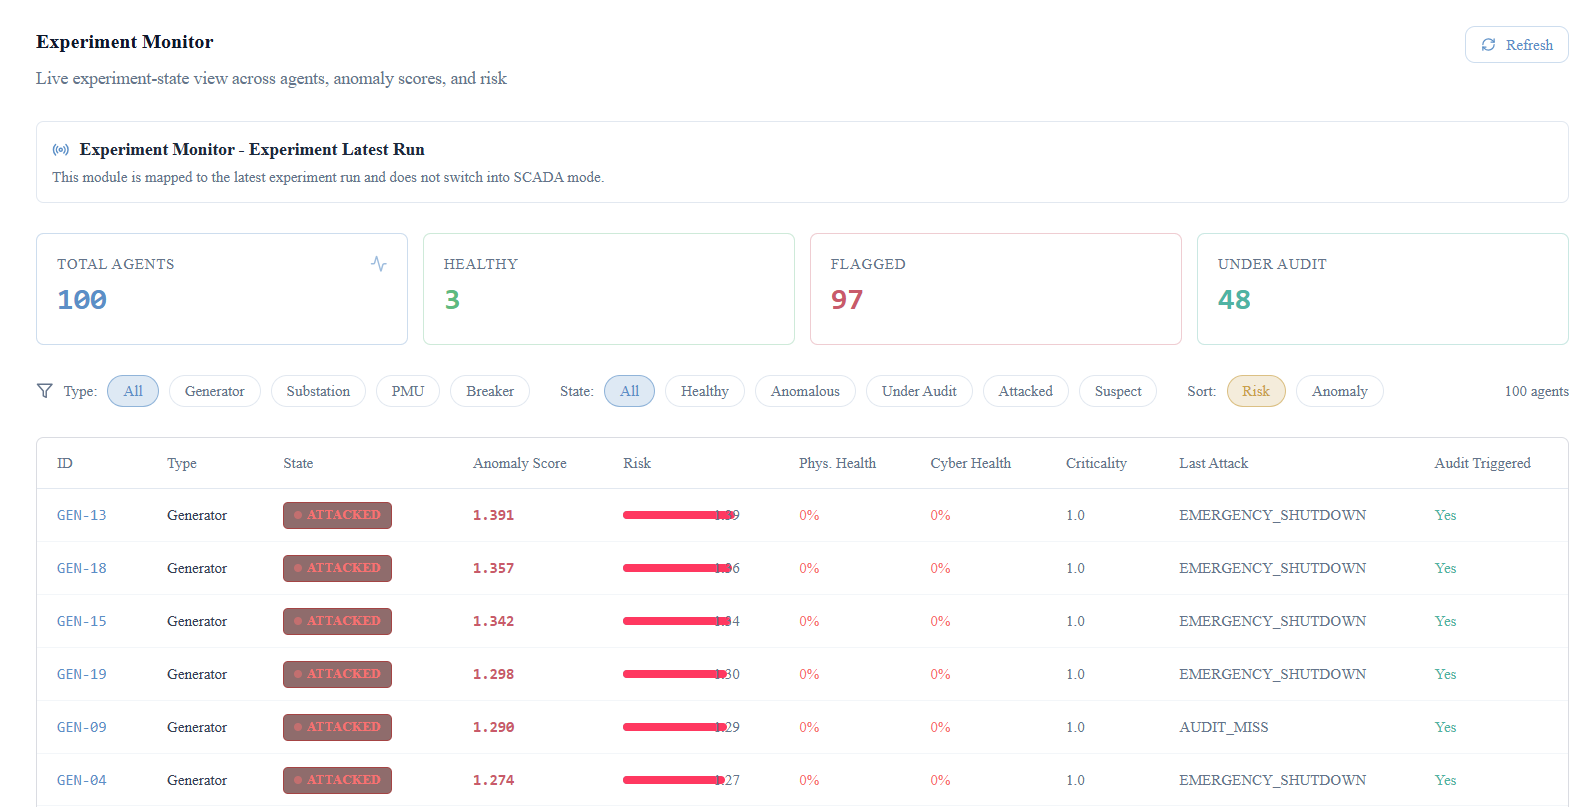
\includegraphics[width=0.95\textwidth]{FigExperiment_Monitor.png}}
\caption{Experiment workspace real-time monitor view displaying live telemetry readings and agent status indicators.}
\label{fig:experiment_monitor}
\end{figure}

\begin{figure}[H]
\centering
\fbox{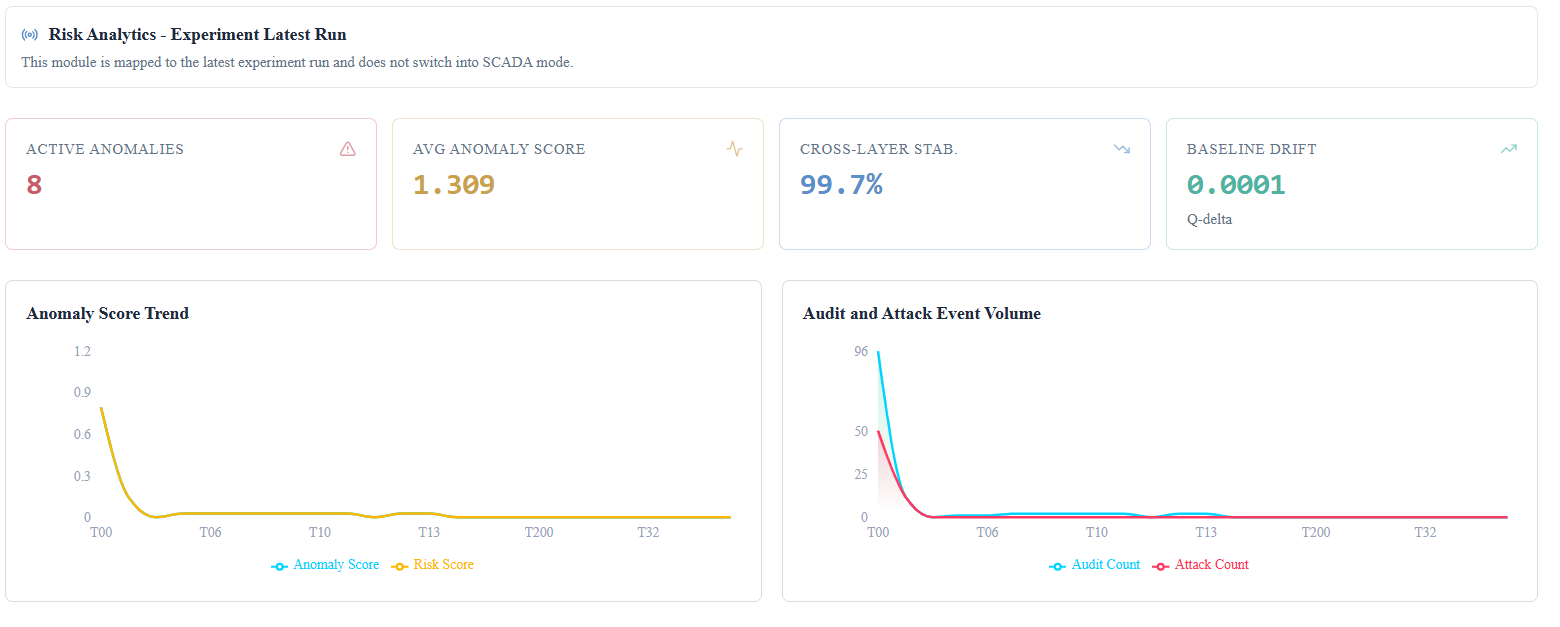
\includegraphics[width=0.95\textwidth]{FigExperiment_Risk_Analytics.png}}
\caption{Risk analytics view from the experiment workspace showing aggregated risk scores and distributions across the agent population.}
\label{fig:experiment_risk_analytics}
\end{figure}

\begin{figure}[H]
\centering
\fbox{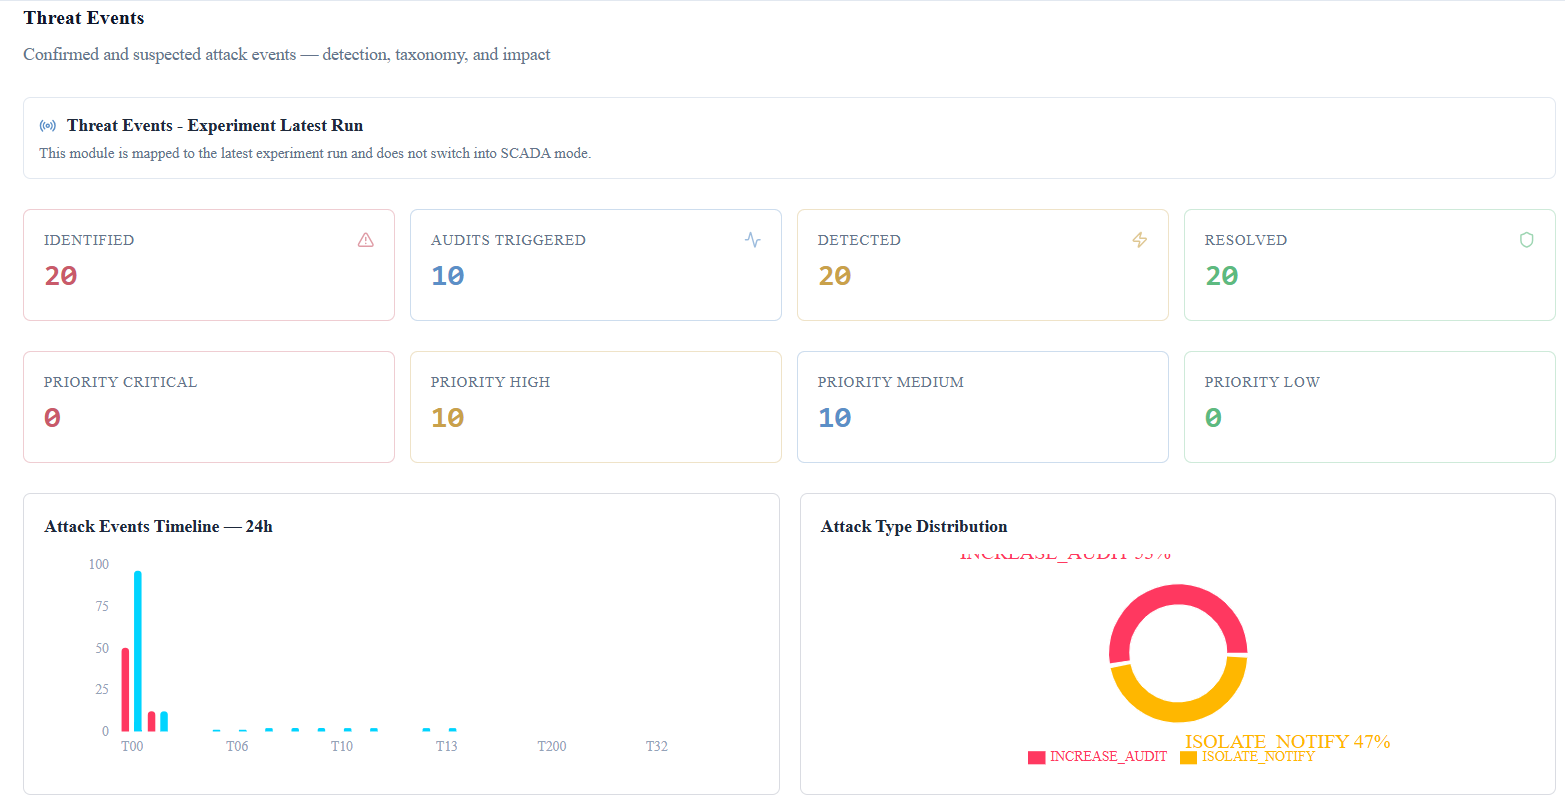
\includegraphics[width=0.95\textwidth]{FigExperiment_Threat_Events.png}}
\caption{Threat events feed from the experiment workspace showing detected anomalies and attack classifications with timestamps.}
\label{fig:experiment_threat_events}
\end{figure}

\begin{figure}[H]
\centering
\fbox{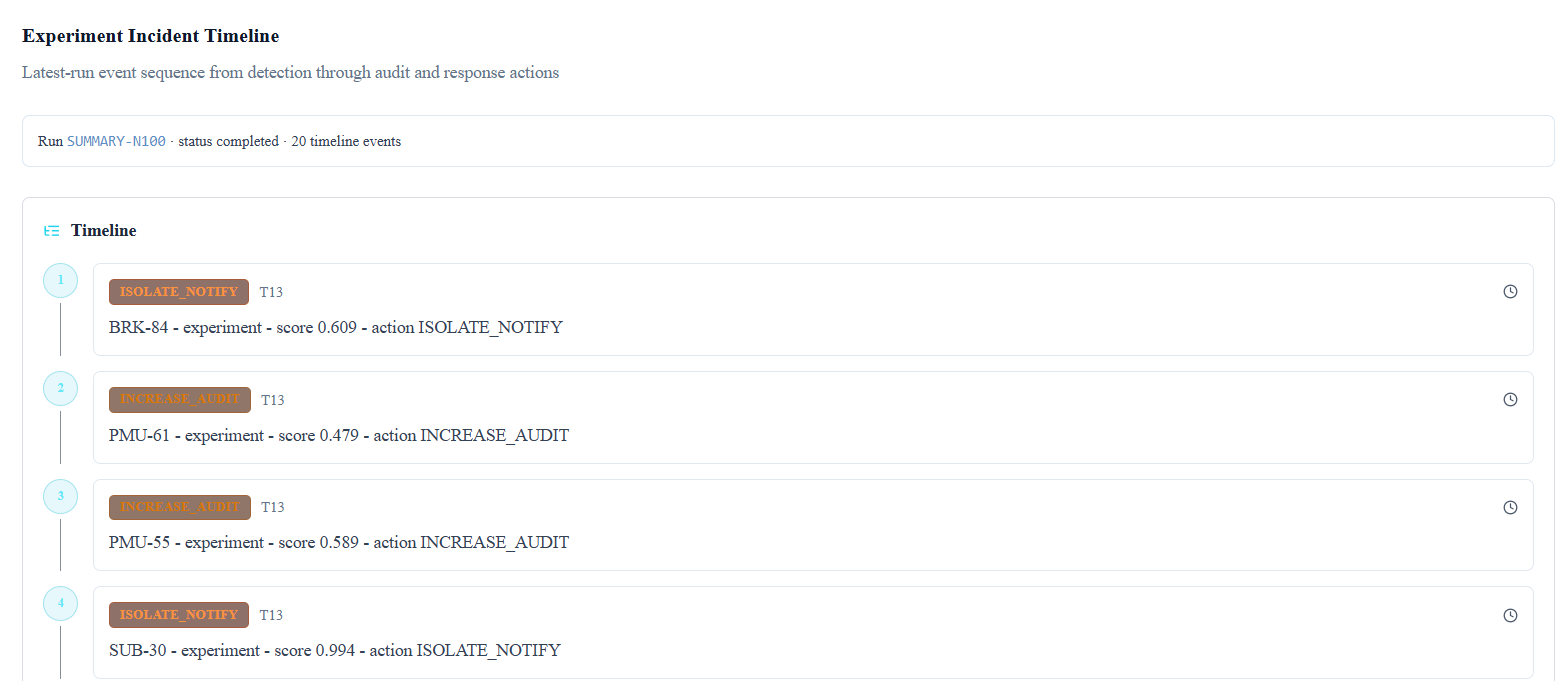
\includegraphics[width=0.95\textwidth]{FigExperiment_Timeline.png}}
\caption{Experiment workspace timeline view showing temporal distribution of anomaly events and audit actions across the simulation horizon.}
\label{fig:experiment_timeline}
\end{figure}

\begin{figure}[H]
\centering
\fbox{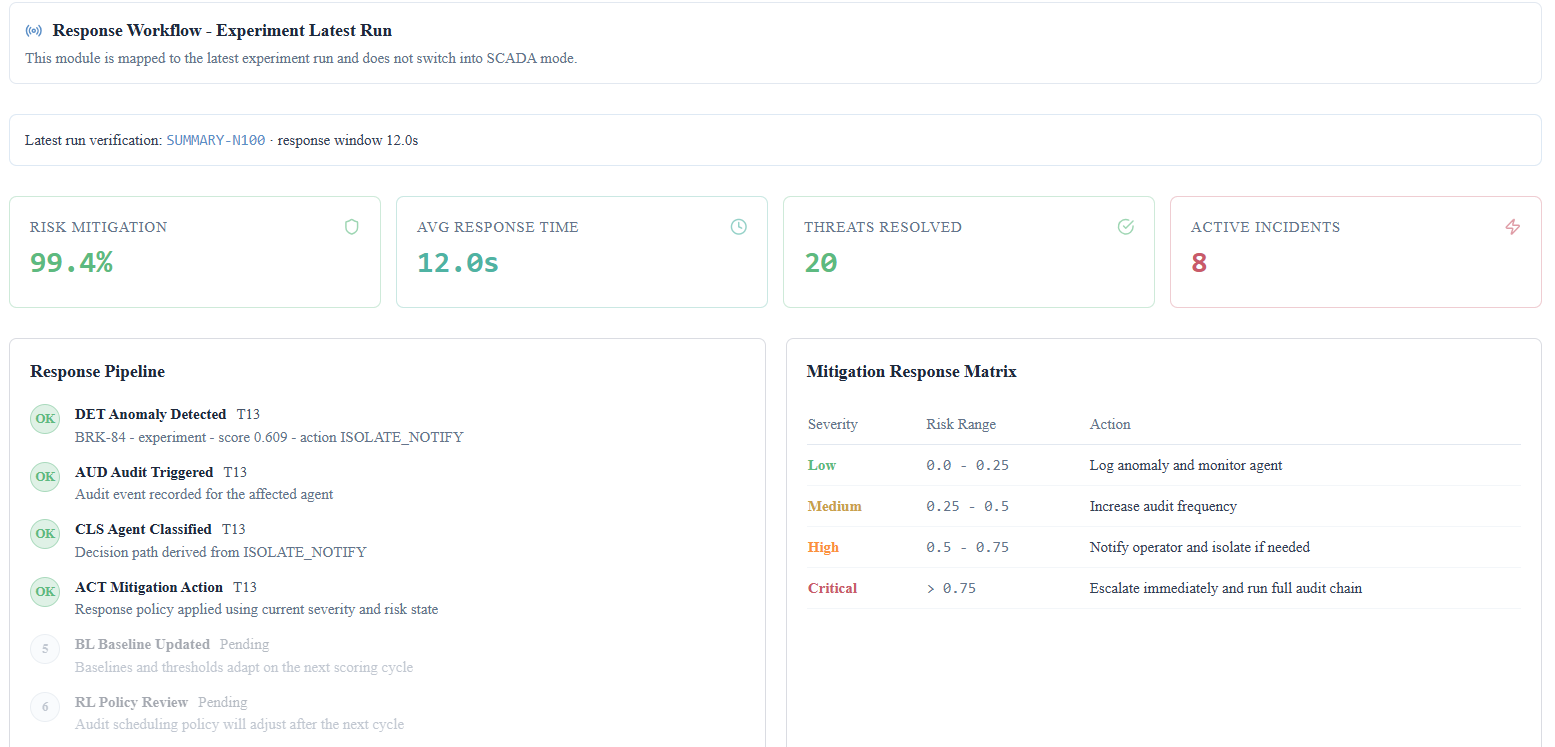
\includegraphics[width=0.95\textwidth]{FigExperiment_Response_Workflow.png}}
\caption{Response workflow view from the experiment workspace showing the current escalation state and sequence of actions for each agent.}
\label{fig:experiment_response_workflow}
\end{figure}

\begin{figure}[H]
\centering
\fbox{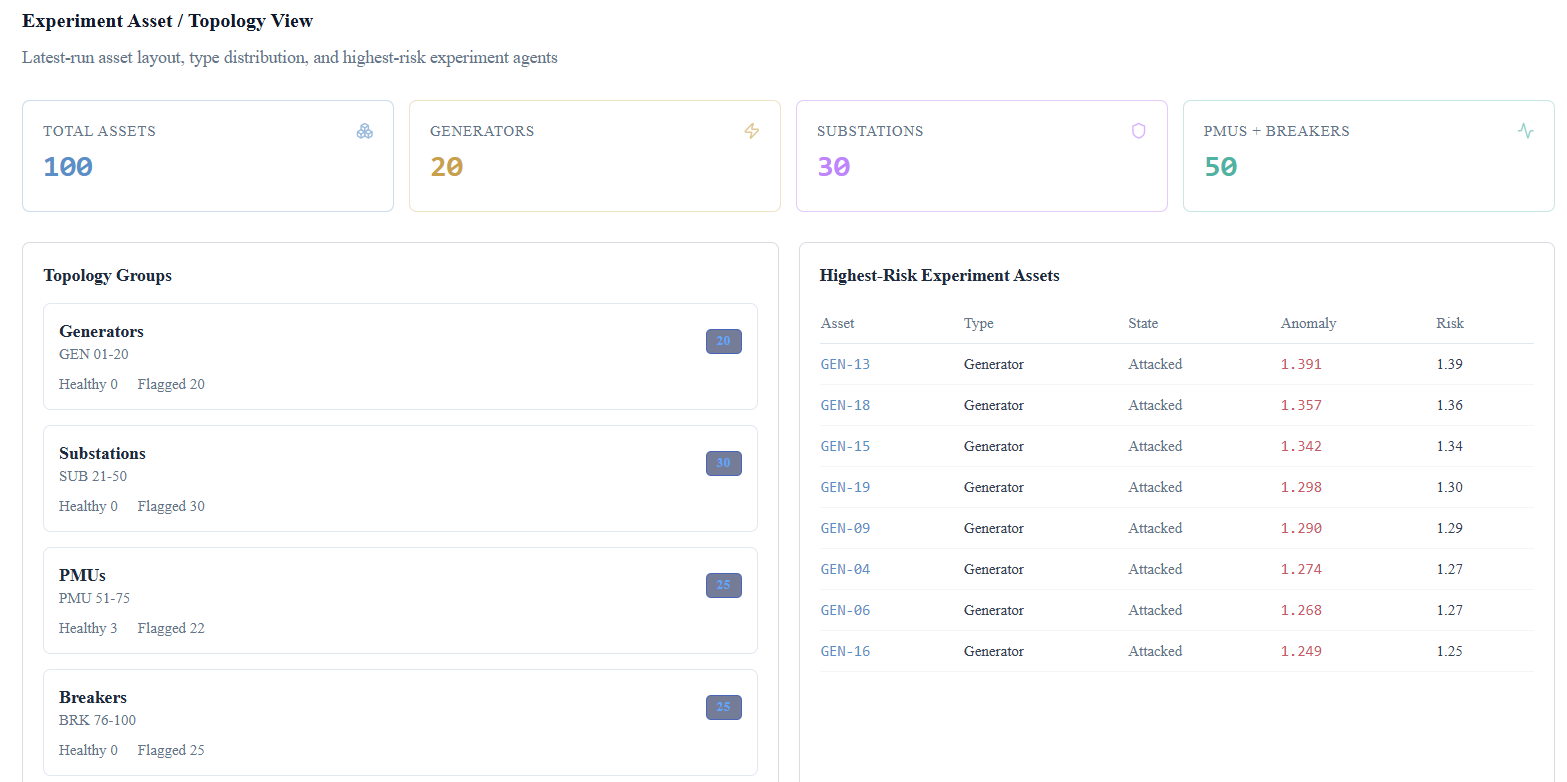
\includegraphics[width=0.95\textwidth]{FigExperiment_Asset_Topology_View.png}}
\caption{Asset topology view from the experiment workspace showing the graphical layout of agents and their inter-relationships.}
\label{fig:experiment_asset_topology}
\end{figure}

\begin{figure}[H]
\centering
\fbox{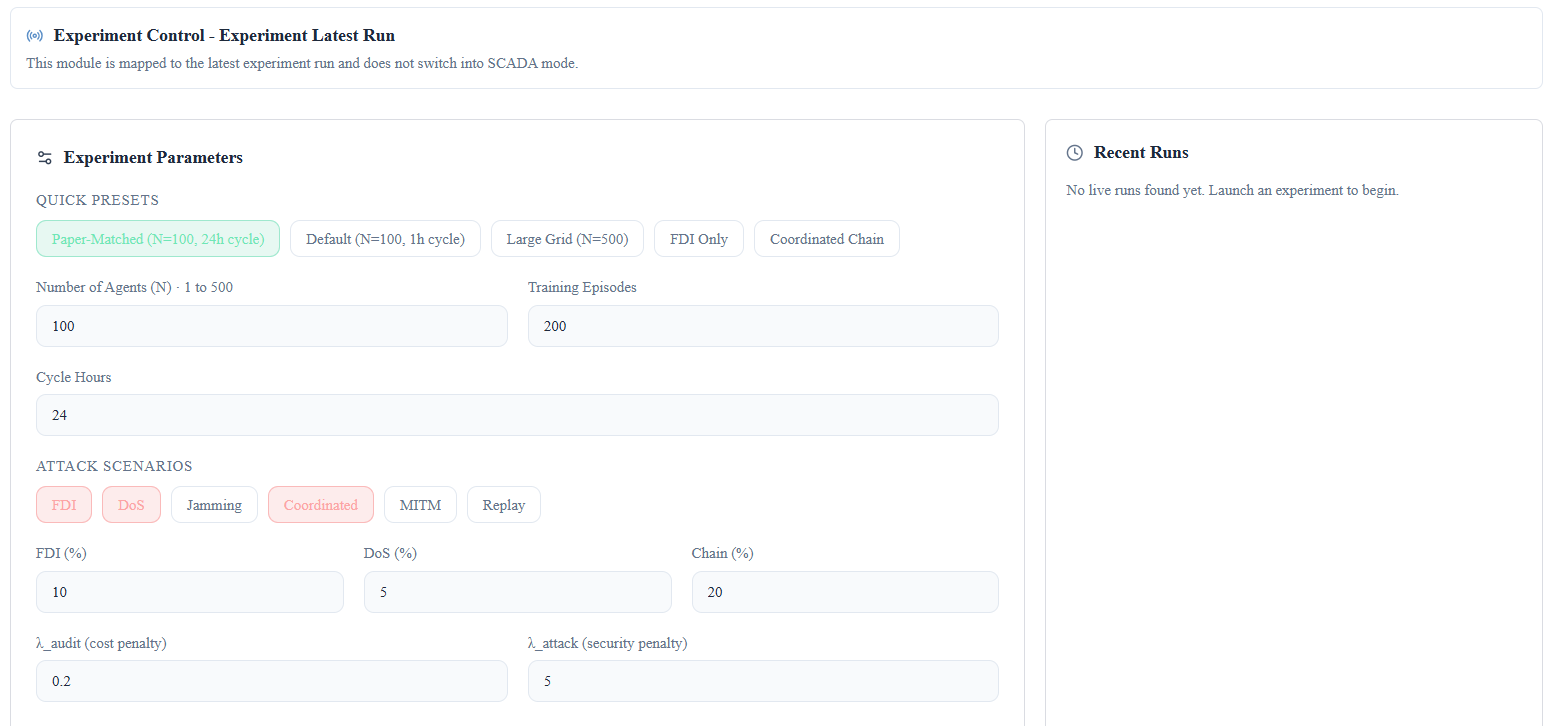
\includegraphics[width=0.95\textwidth]{FigExperiment_Control.png}}
\caption{Experiment control panel providing configuration and execution controls for launching, parameterising, and monitoring experiments.}
\label{fig:experiment_control}
\end{figure}

\par \vspace{0.35cm}
\noindent
Figures~\ref{fig:scada_ops_overview}--\ref{fig:scada_incident_timeline} present the dashboard views from the Rapid SCADA live workspace.

\begin{figure}[H]
\centering
\fbox{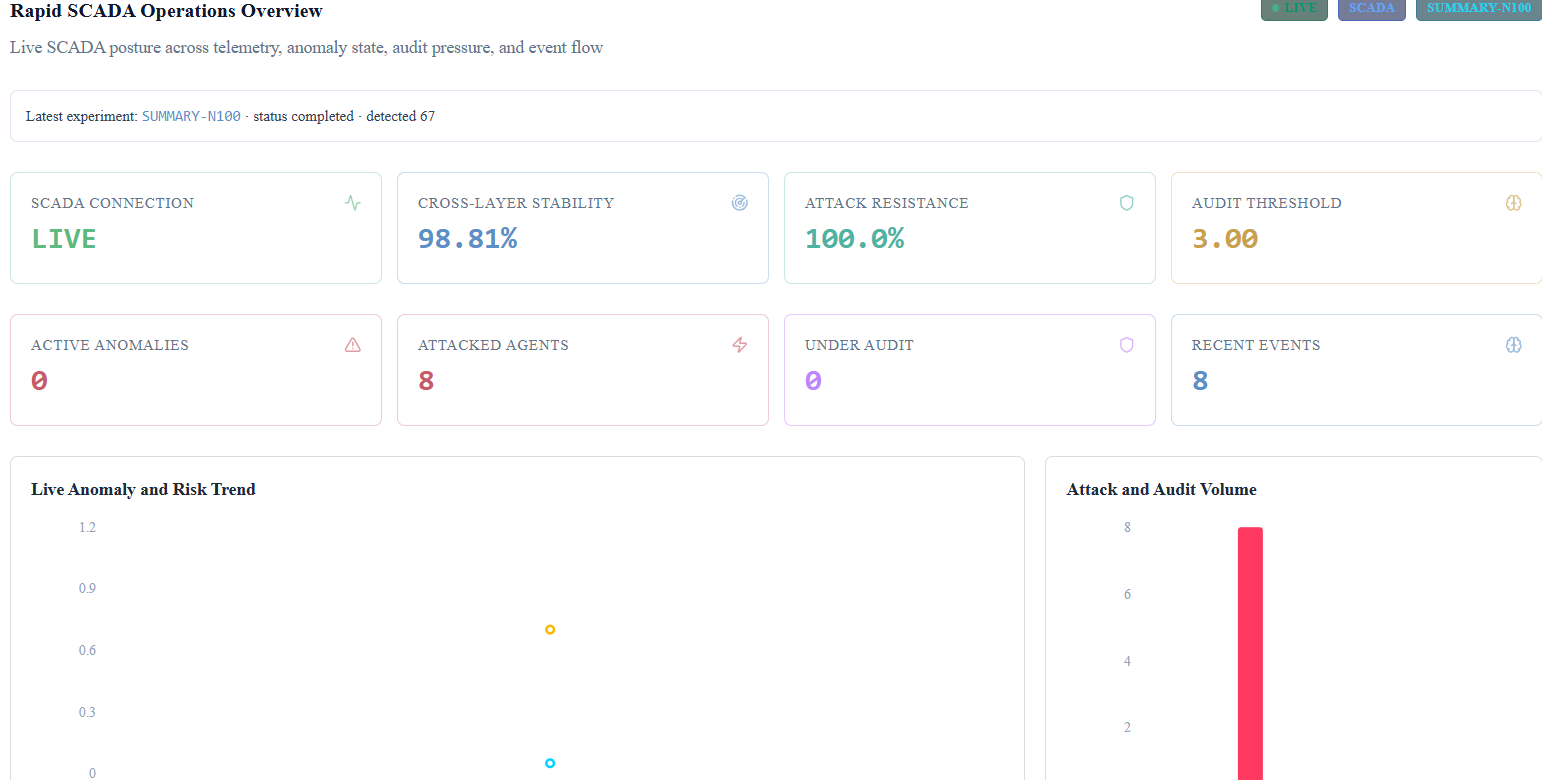
\includegraphics[width=0.95\textwidth]{FigRapid_SCADA_Operations_Overview.png}}
\caption{Rapid SCADA live workspace operations overview showing real-time monitoring status for the 100-agent grid.}
\label{fig:scada_ops_overview}
\end{figure}

\begin{figure}[H]
\centering
\fbox{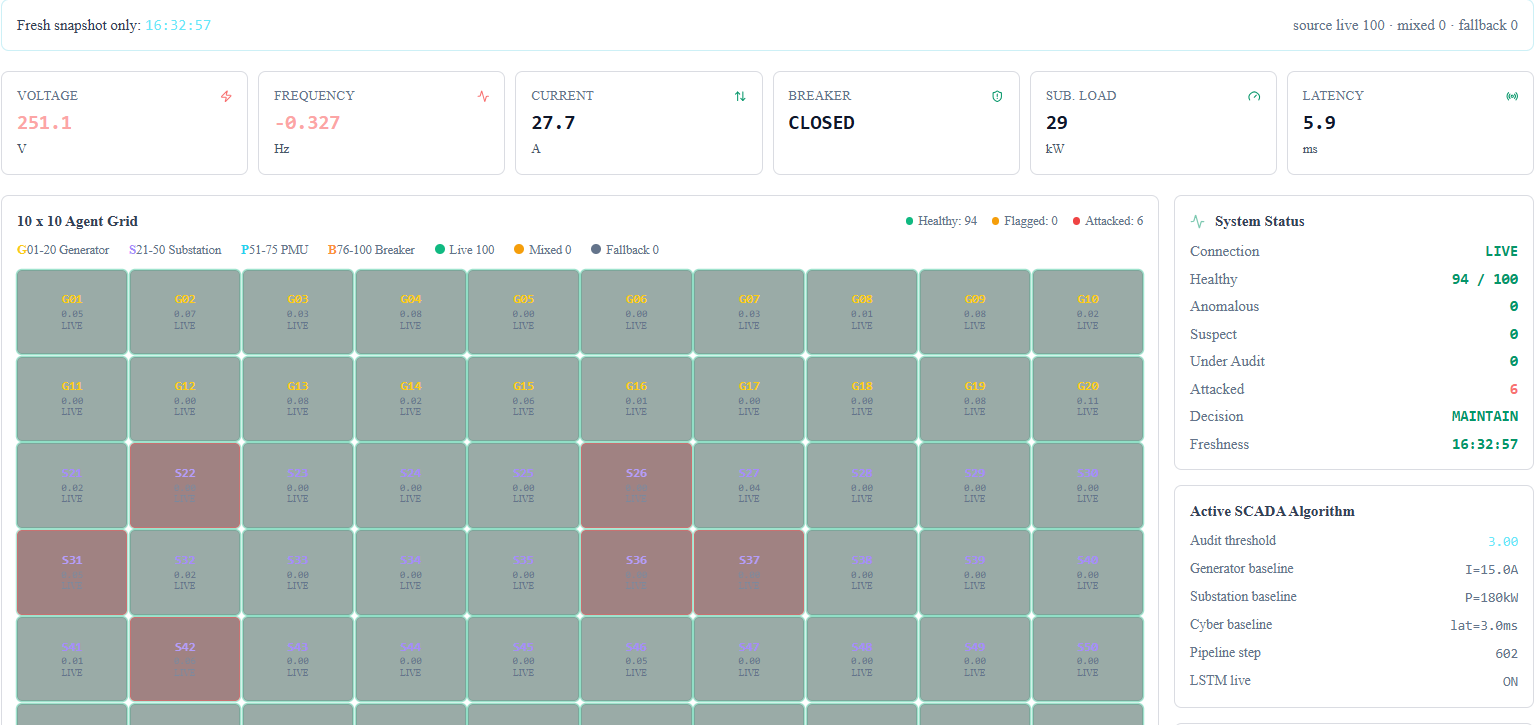
\includegraphics[width=0.95\textwidth]{FigGrid_With_The_Agents.png}}
\caption{SCADA grid view with 100 agents distributed across four asset classes.}
\label{fig:scada_grid_agents}
\end{figure}

\begin{figure}[H]
\centering
\fbox{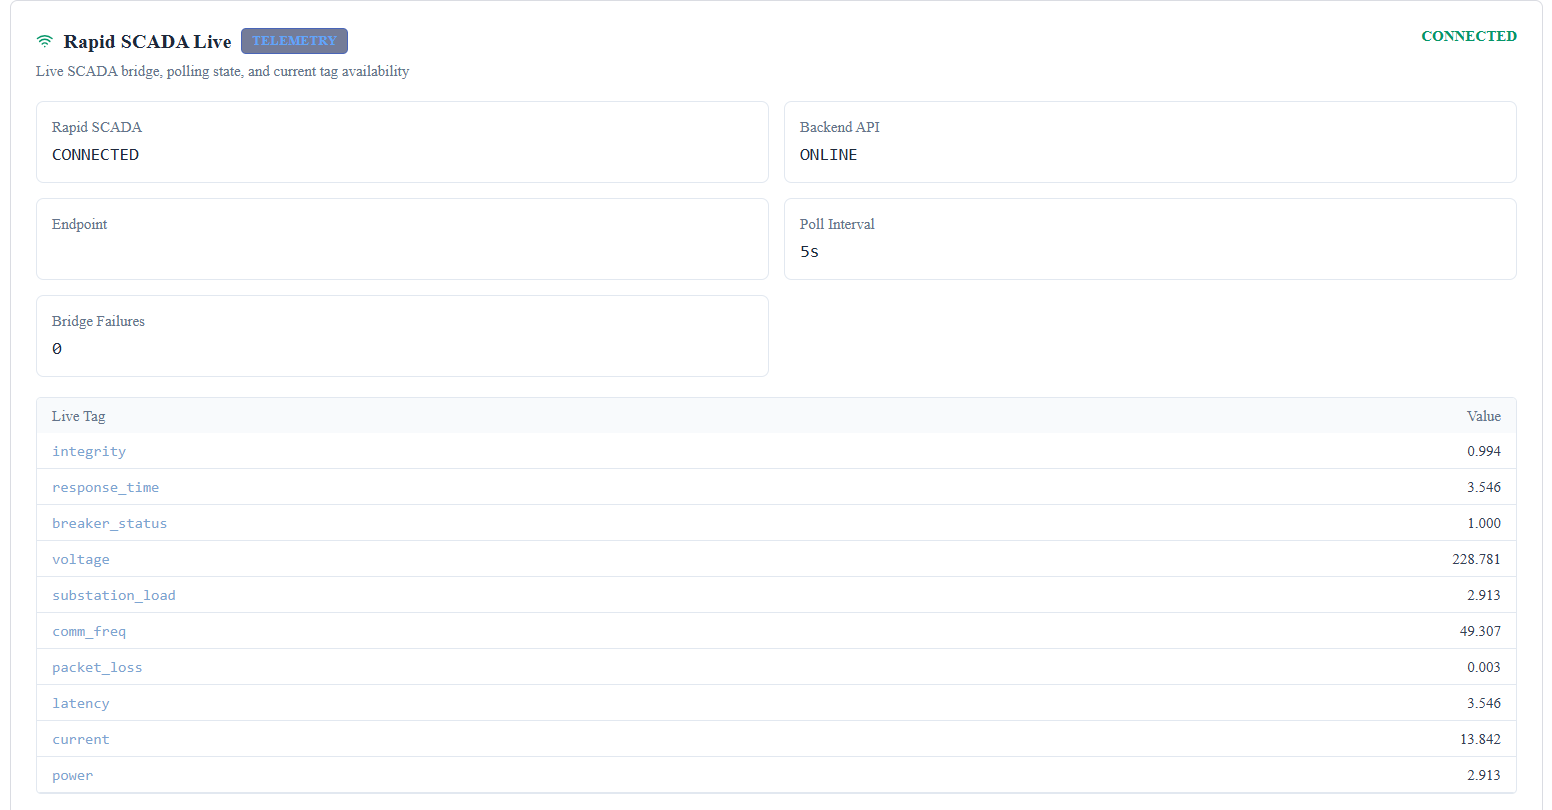
\includegraphics[width=0.95\textwidth]{FigRapid_SCADA_Connectivity.png}}
\caption{Connectivity status panel from the SCADA live workspace showing the health of communication links and bridge connection status.}
\label{fig:scada_connectivity}
\end{figure}

\begin{figure}[H]
\centering
\fbox{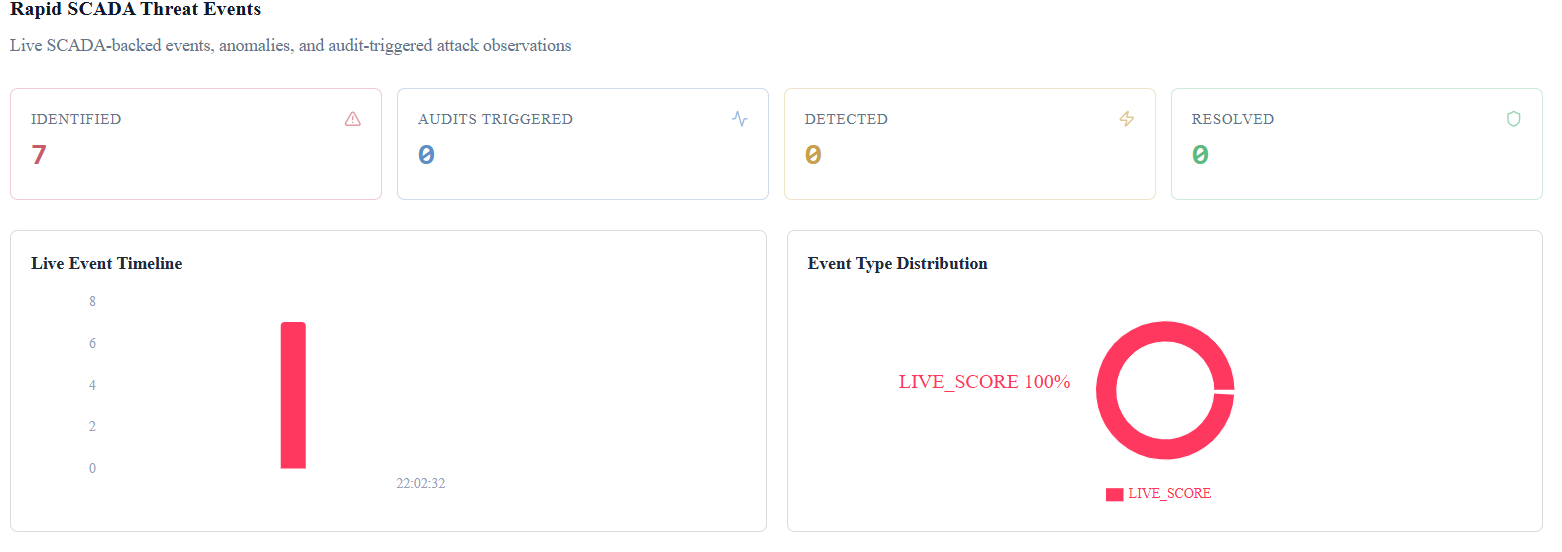
\includegraphics[width=0.95\textwidth]{FigRapid_SCADA_Threat_Events.png}}
\caption{Threat events feed from the SCADA live workspace displaying detected anomalies and their severity levels in real time.}
\label{fig:scada_threat_events}
\end{figure}

\begin{figure}[H]
\centering
\fbox{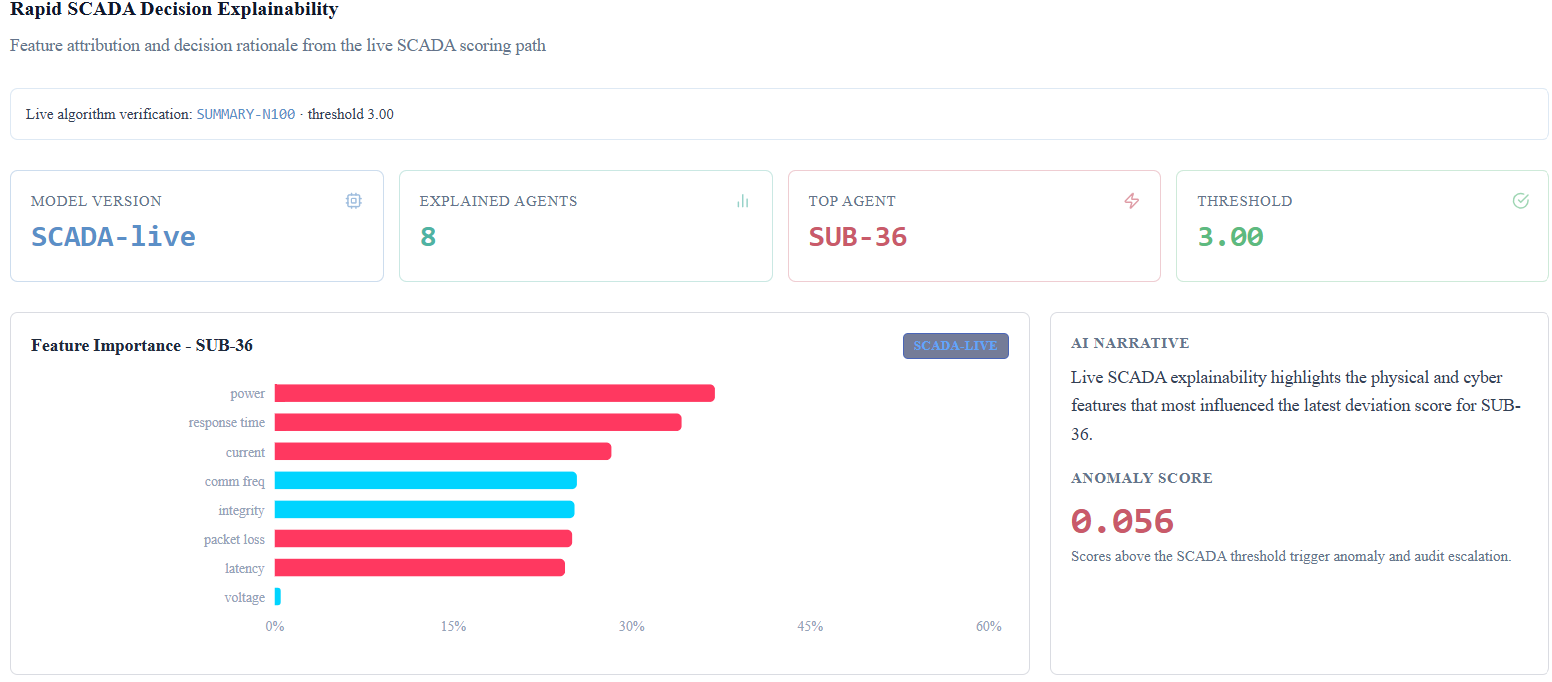
\includegraphics[width=0.95\textwidth]{FigRapid_SCADA_Decision_Explainability.png}}
\caption{Decision explainability view from the SCADA live workspace showing per-feature contribution rankings for a selected agent.}
\label{fig:scada_decision_xai}
\end{figure}

\begin{figure}[H]
\centering
\fbox{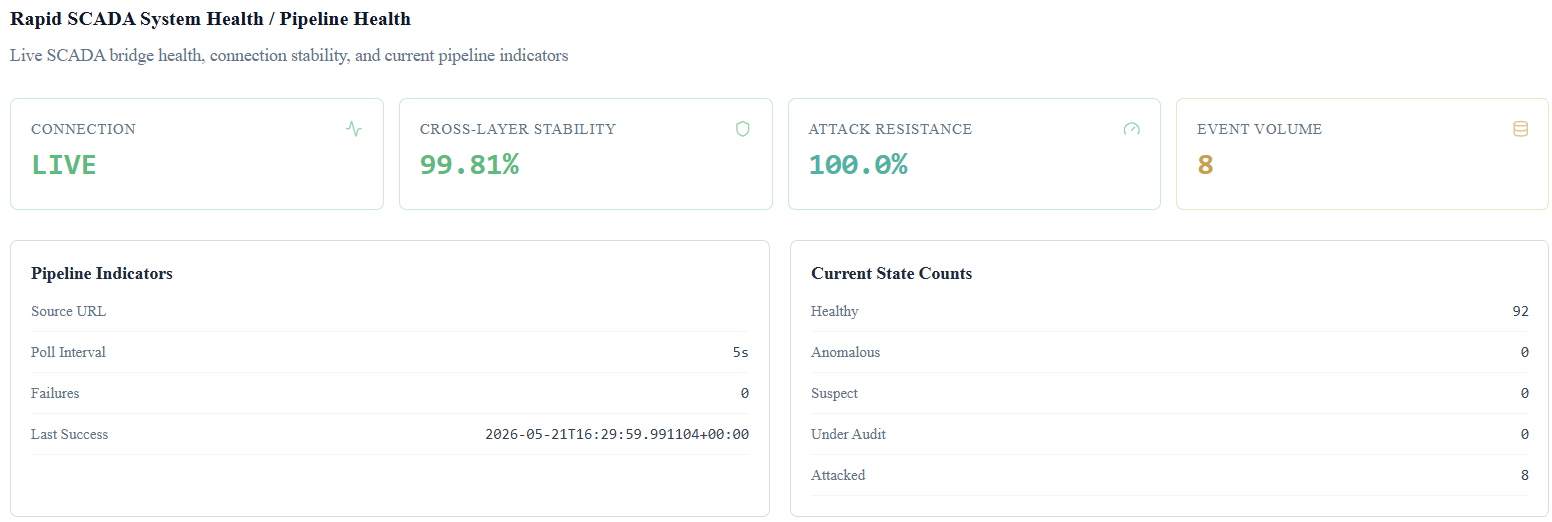
\includegraphics[width=0.95\textwidth]{FigRapid_SCADA_System_Health.png}}
\caption{System health view from the SCADA live workspace showing real-time status indicators for each subsystem component.}
\label{fig:scada_system_health}
\end{figure}

\begin{figure}[H]
\centering
\fbox{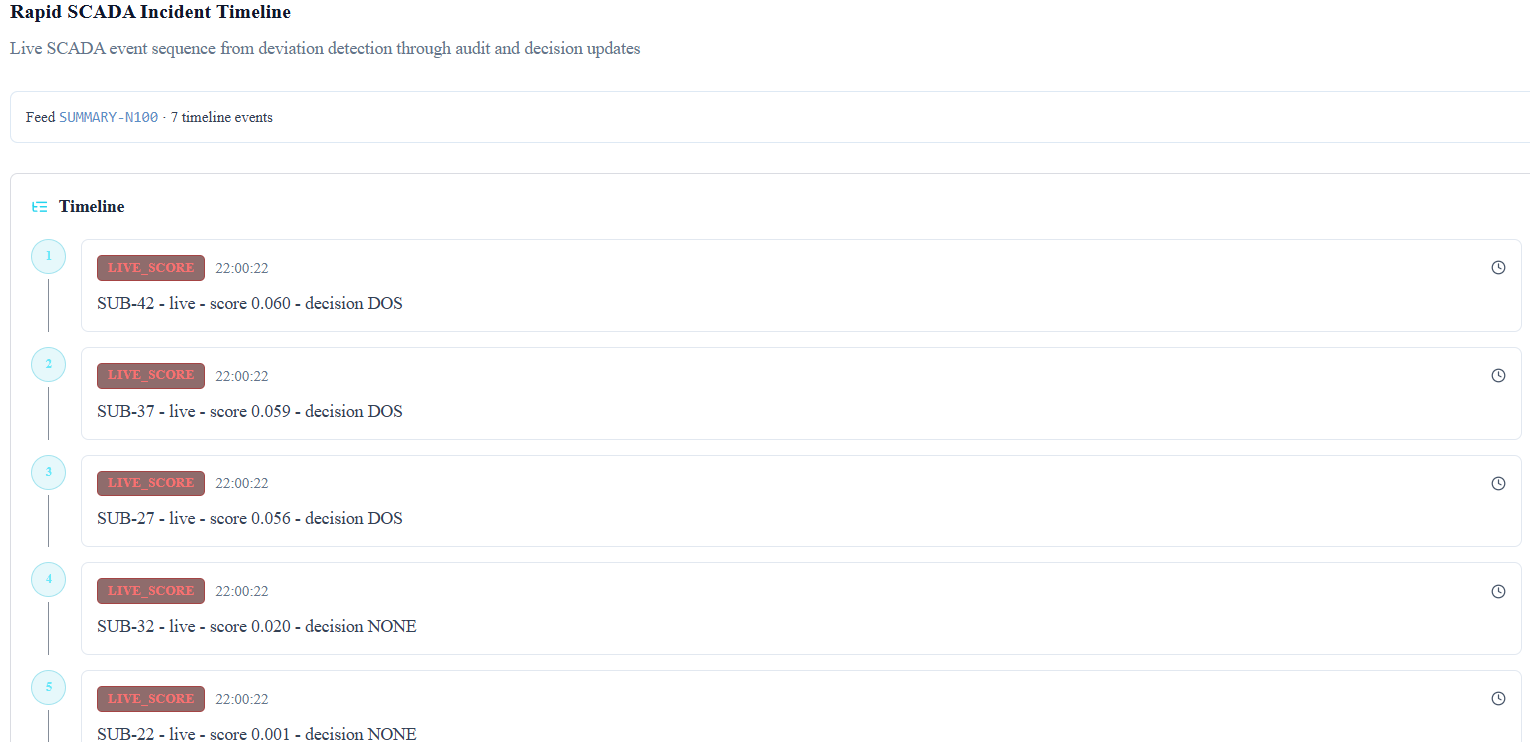
\includegraphics[width=0.95\textwidth]{FigRapid_SCADA_Incident_Timeline.png}}
\caption{Incident timeline view from the SCADA live workspace showing the chronological sequence of detected security events.}
\label{fig:scada_incident_timeline}
\end{figure}

\begin{figure}[H]
\centering
\fbox{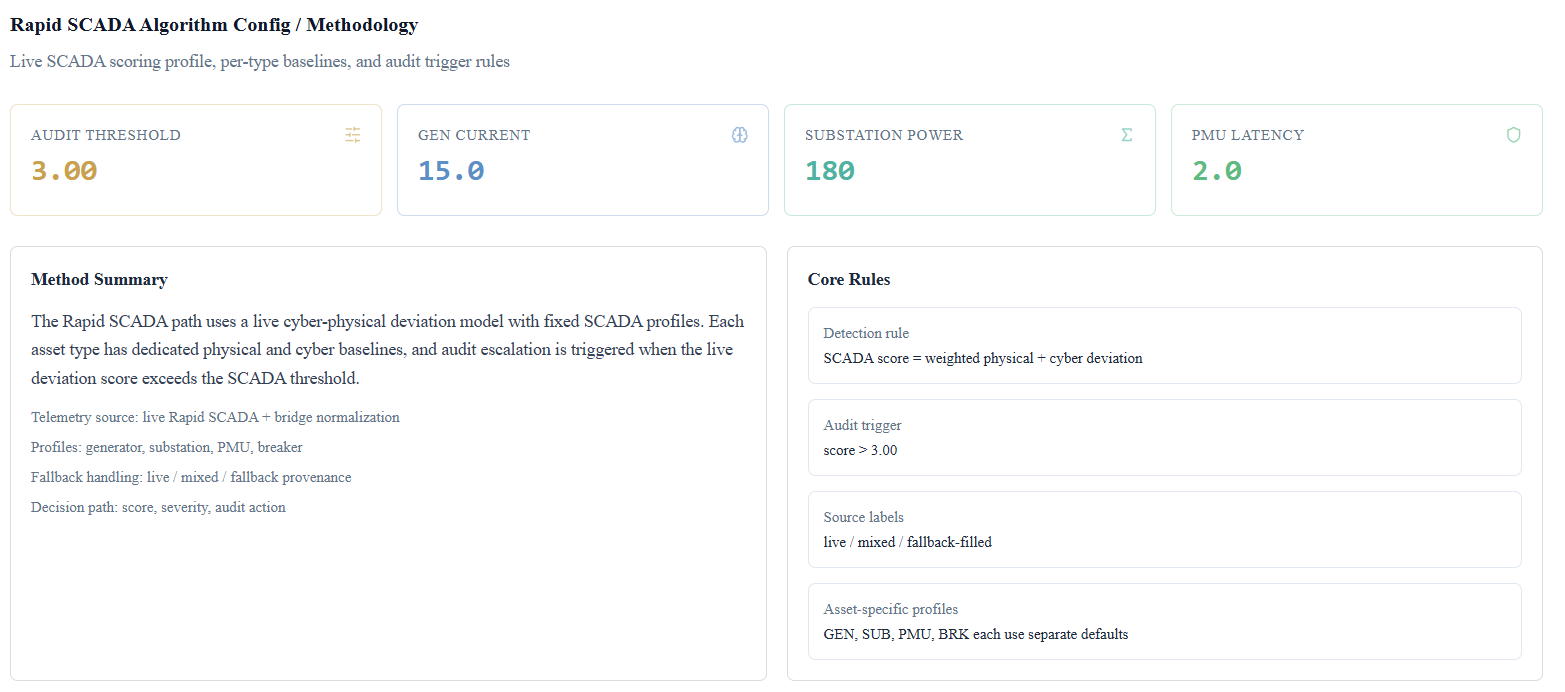
\includegraphics[width=0.95\textwidth]{FigRapid_SCADA_Algorithm_Config_Methodology.png}}
\caption{Algorithm configuration and methodology view from the SCADA live workspace showing the detection pipeline settings.}
\label{fig:scada_algo_config}
\end{figure}

% ============================================================
\section{Operational Workflow}
% ============================================================

The operational workflow of the SmartGrid AI Audit Framework is organised into four sequential phases that correspond to the passage of data through the four architectural tiers.

\par \vspace{0.35cm}
\textbf{Phase I: Data Acquisition.} In the first phase, raw telemetry is acquired from the active data source. In the experiment workspace, data is generated by the backend simulation engine according to the configured scenario parameters. In the SCADA live workspace, data is retrieved from the Rapid SCADA server through the PowerShell bridge. Regardless of source, the raw observations are validated, timestamped, and queued for processing.

\par \vspace{0.35cm}
\textbf{Phase II: Feature Preparation.} In the second phase, each raw observation is decomposed into its physical and cyber feature components. Physical features (voltage, current, frequency, power, response time) and cyber features (latency, packet loss, communication frequency, integrity) are extracted and normalised against their type-specific baselines using the transformation defined in Equation~\ref{eq:normalisation}. The result is a standardised feature vector for each agent at each timestep.

\par \vspace{0.35cm}
\textbf{Phase III: Multi-Layer Anomaly Evaluation.} In the third phase, the normalised feature vectors are processed by the multi-layer detection engine. The statistical deviation scorer computes instantaneous deviation scores. The LSTM temporal detector processes the 24-timestep sliding window to produce calibrated anomaly probabilities. The weighted ensemble fuses these outputs into hybrid confidence values. Simultaneously, the three-layer multi-detector architecture evaluates the agent against the calibrated threshold (Layer~A), the temporal accumulator (Layer~B), and the attack-specific detectors for FDI, DoS, and MITM (Layer~C). The OR-with-precedence combiner produces the final anomaly determination, and the false positive suppression mechanism filters low-confidence detections.

\par \vspace{0.35cm}
\textbf{Phase IV: Hybrid Audit Decision and Output.} In the fourth phase, the detection outputs are consumed by the hybrid audit scheduler, which determines the appropriate audit frequency and escalation action for each agent using Q-learning and gradient-based cost optimisation under budget constraints. The explainability module generates per-agent reason codes and feature contribution rankings. All outputs, anomaly flags, risk scores, escalation actions, and explanations, are pushed to the visualisation layer for operator consumption and are simultaneously logged to the audit trail for traceability.

% ============================================================
\section{Research Contributions}
% ============================================================

The proposed SmartGrid AI Audit Framework makes the following research and engineering contributions:

\begin{enumerate}
    \item \textbf{Unified Cyber-Physical Framework:} A single platform that combines multi-layer anomaly detection, hybrid audit decision support, per-feature explainability, and live SCADA integration within a single modular architecture.

    \item \textbf{Multi-Layer Detection with Ensemble Fusion:} A detection methodology that combines statistical deviation scoring with LSTM-based temporal analysis through a weighted ensemble (deviation weight 0.48, LSTM probability weight 0.52), producing calibrated hybrid confidence estimates.

    \item \textbf{Three-Layer Multi-Detector for Attack Classification:} A specialised detection architecture comprising a calibrated LSTM threshold (Layer~A), a temporal accumulator (Layer~B), and attack-specific detectors for false data injection via CUSUM, denial of service via rule-based corroboration, and man-in-the-middle via integrity-jump analysis (Layer~C).

    \item \textbf{Hybrid Audit Scheduling under Budget Constraints:} A scheduling mechanism that combines Q-learning-based frequency adjustment with gradient-based cost optimisation to determine cost-efficient audit strategies while enforcing operational budget limits.

    \item \textbf{Dual-Workspace Separation:} A clear architectural separation between the experiment evaluation environment and the live operational monitoring environment, so that benchmarking and production monitoring can run independently over a shared detection and audit engine.

    \item \textbf{End-to-End SCADA Telemetry Path:} A fully operational data pipeline from Rapid SCADA through a PowerShell bridge to the FastAPI backend, showing real SCADA-to-backend telemetry acquisition and processing in action.

    \item \textbf{Live 100-Agent Deployment:} A live deployment spanning 100 agents across four distinct asset classes, generators, substations, phasor measurement units, and breakers, each with type-specific baselines and feature definitions.

    \item \textbf{Explainable Scoring with Feature Contribution Ranking:} A per-agent, per-timestep explainability mechanism that computes relative feature contributions independently for physical and cyber domains, producing human-readable reason codes for every detection.

    \item \textbf{Five-Method Comparative Validation Study:} A comparative evaluation of the proposed multi-layer approach against deviation-only, LSTM-only, Isolation Forest, and One-Class SVM baselines, which confirms the value of the ensemble and multi-detector design.

    \item \textbf{From Conceptual Framework to Functioning Platform:} An extension of the foundational base paper from a conceptual cyber-physical audit framework to a fully implemented, integrated, and deployable software platform with real-time monitoring, detection, and decision support capabilities.

    \item \textbf{Five-Class Attack Typing with Temporal Signature Analysis:} An attack classification layer that assigns each flagged agent one of five attack type labels (FDI, DoS, MITM, Physical Fault, and Coordinated Chain Attack) by combining Layer~C detector outputs with a lightweight temporal signature classifier that recognises STEP, RAMP, OSCILLATORY, and STABLE deviation patterns.

    \item \textbf{Dual-Dataset LSTM Pre-Training Pipeline:} A pre-training methodology that initialises the physical grid branch using the UCI Electrical Grid Stability Dataset and the cyber network branch using the UNSW-NB15 Network Intrusion Dataset, with engineered composite features that map directly onto the simulation's cyber feature space. This pre-training step gives each LSTM branch meaningful starting weights before fine-tuning on synthetic grid data.
\end{enumerate}
